% =====================================================================
%  Chapter 3 — Internship Activities
%  Structure fixed by docs/guidelines/guidelines.md (section 3, item 3):
%    3.1 Roles and Responsibilities
%    3.2 Weekly log
%    3.3 Description of the Project(s) Involved During Internship
%    3.4 Tasks / Activities Performed
%  Note the order: the guidelines put the weekly log BEFORE the project
%  description. Sample 1 uses a different order; follow the guidelines.
%
%  Content sources: docs/project_detail/11_report_mapping.md (Chapter 3)
% =====================================================================
\chapter{Internship Activities}

% ---------------------------------------------------------------------
\section{Roles and Responsibilities}
During the twelve-week internship at Power Gym Budibazar Pokhara, the intern was assigned the designation of Mobile Application Developer Intern within the Digitalization Unit. The intern's primary technical mandate centered on frontend software engineering, user interface implementation, and visual design system integration for the Alcedo mobile fitness application. In addition to client-side duties, the intern contributed to supporting backend service development, data model management, and frontend--backend integration workflows.

The specific responsibilities fulfilled during the internship encompassed four core technical areas:
\begin{itemize}
    \item \textbf{Frontend Development and User Interface Implementation:} Constructing application screens and modular interface components, including responsive layouts, action buttons, interactive cards, input form controls, typography scales, dynamic spacing, and client navigation transitions. The primary focus was delivering a pixel-accurate, consistent user interface adhering strictly to design specifications across varying mobile screen viewports.
    \item \textbf{Backend Development and Data Management:} Contributing to modular backend services within the newer NestJS architecture, specifically focusing on User Management, Workout Management, and Feature Management. Responsibilities included developing endpoints for retrieving and updating user profile information, building Create, Read, Update, and Delete (CRUD) operations for workout sessions and exercise logs, and establishing data validation rules.
    \item \textbf{Frontend--Backend Integration and Feature Control:} Connecting frontend UI components with backend RESTful endpoints, managing asynchronous data flow, implementing loading and error states, and integrating runtime feature flags to toggle application capabilities dynamically via server-side configuration.
    \item \textbf{Software Verification, Debugging, and Quality Assurance:} Conducting comprehensive component testing, verifying screen flows on mobile emulators, executing unit test suites, performing static type checking, identifying runtime anomalies, and systematically resolving defects.
\end{itemize}

A structured breakdown mapping the intern's assigned responsibilities to concrete technical activities and delivered outcomes is presented in Table~\ref{tab:roles-summary}.

\begin{table}[htbp]
    \centering
    \caption{Summary of Roles and Assigned Responsibilities}
    \label{tab:roles-summary}
    \begin{tabular}{|p{1.8in}|p{4.2in}|}
        \hline
        \textbf{Responsibility Area} & \textbf{Technical Activities and Deliverables} \\
        \hline
        Frontend Development \& UI Engineering & Implemented 24 tracked mobile route screens across 5 core navigation tabs; constructed over 80 reusable design foundation components (buttons, input fields, cards, dialogs) adhering to centralized design tokens. \\
        \hline
        Client Architecture \& State Management & Structured file-based routing using Expo Router; centralized client state with 11 Redux Toolkit slices; configured listener middleware for non-blocking persistence. \\
        \hline
        Embedded Storage \& Data Persistence & Designed local SQLite schemas managed via Drizzle ORM across 17 database tables; implemented sequential SQL schema migrations; configured hardware-backed secure storage. \\
        \hline
        Backend Service Engineering & Implemented User Management (\textit{PATCH /api/users/me}), Workout Management (CRUD and batch sync contracts), and Feature Management flags in NestJS 11 and MongoDB 8. \\
        \hline
        Frontend--Backend Integration & Engineered an authenticated network client wrapper (\textit{authenticated-fetch}) featuring single-flight 401 token refresh interceptors, JWT lifecycle rotation, and service probe checks. \\
        \hline
        Quality Assurance \& Defect Resolution & Executed automated Vitest test suites (140 spec files), component simulation suites, strict TypeScript typechecking, and iterative debugging against quality gates. \\
        \hline
    \end{tabular}
\end{table}

Through these responsibilities, the intern successfully applied theoretical principles acquired during the B.Sc. CSIT curriculum---including software engineering lifecycles, database normalization, object-oriented design, and network protocols---to a production-grade mobile software application, acquiring practical proficiency in professional software development methodologies.

% ---------------------------------------------------------------------
\section{Weekly Log}
In accordance with the curriculum requirements of Tribhuvan University, a chronological record of technical activities performed throughout the twelve-week internship was maintained. The technical tasks, system observations, and engineering milestones are summarized in Table~\ref{tab:weekly-logs}.

\begin{longtable}{|c|p{1.4in}|p{2.3in}|p{1.7in}|}
    \caption{Weekly Log of Internship Activities}\label{tab:weekly-logs}\\
    \hline
    \textbf{Week} & \textbf{Responsibilities} & \textbf{Activities Performed} & \textbf{Observations} \\
    \hline
    \endfirsthead
    \multicolumn{4}{c}%
    {\textbf{Table \ref{tab:weekly-logs}: Continued from previous page}} \\
    \hline
    \textbf{Week} & \textbf{Responsibilities} & \textbf{Activities Performed} & \textbf{Observations} \\
    \hline
    \endhead
    \hline
    \multicolumn{4}{r}{\textit{Continued on next page}} \\
    \endfoot
    \hline
    \endlastfoot
    1 & Onboarding and orientation & Met with company mentor and organizational team; reviewed the functional objectives and architectural scope of the Alcedo application; configured local development environment, Node.js runtimes, package managers, and Git repository access. & Gained clarity regarding internal software repository structure, development conventions, and project deliverable expectations. \\
    \hline
    2 & Requirements analysis and design planning & Analyzed functional software requirements and provided UI/UX Figma wireframes; evaluated client directory architecture; mapped out the 24 target screen routes across the planned navigation hierarchy. & Thorough upfront architectural analysis and route planning significantly reduce code refactoring in subsequent implementation phases. \\
    \hline
    3 & Reusable component kit and navigation scaffold & Developed atomic design foundation components (buttons, input fields, cards, modal dialogs); established the root navigation layout and primary tab bar hierarchy using Expo Router. & Constructing centralized, reusable UI components establishes visual consistency and accelerates multi-screen development. \\
    \hline
    4 & Frontend screen implementation (Phase 1) & Implemented initial core application screens including the Home dashboard, active workout tracking layouts, set-entry cards, rest timer dialogs, and dynamic spacing tokens. & Establishing strict padding, margin, and typography tokens ensures layout adaptability across diverse device resolutions. \\
    \hline
    5 & Frontend screen implementation (Phase 2) & Implemented remaining application screens, including historical calendar views, session inspection cards, visual strength trends, and user settings interfaces; refined screen navigation transitions. & Maintaining visual coherence across multi-tab routes substantially enhances overall user interface experience and usability. \\
    \hline
    6 & User Management backend and profile UI & Implemented User Management modules in NestJS (\textit{/api/users/me}); built profile retrieval and update endpoints; integrated client-side profile editing screen with backend data handling. & Understood bidirectional data flow, Data Transfer Object (DTO) validation, and client-server synchronization for user profile attributes. \\
    \hline
    7 & Workout UI components and session workflows & Implemented specialized workout interface components for logging exercise sets (warmup, working, failure, drop sets), cardio duration tracking, and dynamic exercise search selection. & Complex list-based data layouts require careful virtualization and memoization to prevent rendering bottlenecks. \\
    \hline
    8 & Workout Management backend services & Developed server-side Workout Management modules in NestJS and MongoDB; implemented CRUD operations for workout sessions and set records; established batch synchronization data contracts. & CRUD operations and atomic database updates form the resilient core of data-driven fitness tracking applications. \\
    \hline
    9 & Feature Management and dynamic flags & Developed Feature Management capabilities in backend-v2 (\textit{GET /api/features}); built client-side capability probe (\textit{backend-probe.ts}) to dynamically toggle application feature modules via server configuration. & Feature flagging decouples code deployment from feature release, enabling flexible runtime configuration without client rebuilds. \\
    \hline
    10 & Frontend--backend integration and error handling & Integrated client network client (\textit{authenticated-fetch}) with backend endpoints; implemented JWT bearer token injection, single-flight 401 refresh interceptors, loading states, and error alerts. & Resilient network interceptors and graceful error handling prevent application crashes and maintain session continuity. \\
    \hline
    11 & Software testing and bug fixing & Executed automated unit tests across frontend Redux slices and components using Vitest; performed regression testing on Android emulators; resolved discovered layout and state anomalies. & Automated testing and static typechecking reveal subtle edge-case state mutations that evade manual inspection. \\
    \hline
    12 & System polish, documentation, and delivery & Conducted comprehensive codebase audit; resolved outstanding interface defects; finalized API and architectural documentation; prepared project artifacts for formal evaluation. & Delivering production-grade software requires disciplined code cleanup, automated gate execution, and clear documentation. \\
\end{longtable}

% ---------------------------------------------------------------------
\section{Description of the Project(s) Involved During Internship}
The technical deliverable developed during the internship is \textbf{Alcedo}, a comprehensive cross-platform mobile fitness platform engineered to modernize athletic training management for Power Gym Budibazar Pokhara. While the software repository historically inherited the open-source base name \textit{LiftLog}, the product identity, bundle configurations, user-facing branding, and server interfaces were customized and advanced under the Alcedo system identity.

\subsection{Product Purpose and Operational Objectives}
The primary objective of Alcedo is to provide gym members with an intuitive, reliable, and offline-capable mobile companion that replaces fragmented paper logs and informal memory with structured digital tracking. From an administrative perspective, the platform provides Power Gym with a modern digital channel to structure verified exercise catalogs, deliver standardized workout blueprints, distribute dynamic configuration updates, and establish member profile services.

The application interface encompasses three primary interactive hubs, as illustrated in Figure~\ref{fig:app-screens}:
\begin{itemize}
    \item \textbf{Home Dashboard:} Displays current workout streaks, quick-start session initiators, weekly training volume summaries, and immediate access to planned routines.
    \item \textbf{Live Workout Execution:} Delivers real-time set recording (weights, reps, RPE, rest intervals), cardio tracking, exercise replacements, and live superset management.
    \item \textbf{Performance Analytics and Trends:} Visualizes historical training volume heatmaps, personal record (PR) milestones, and muscular load distributions across muscle groups.
\end{itemize}

\begin{figure}[htbp]
    \centering
    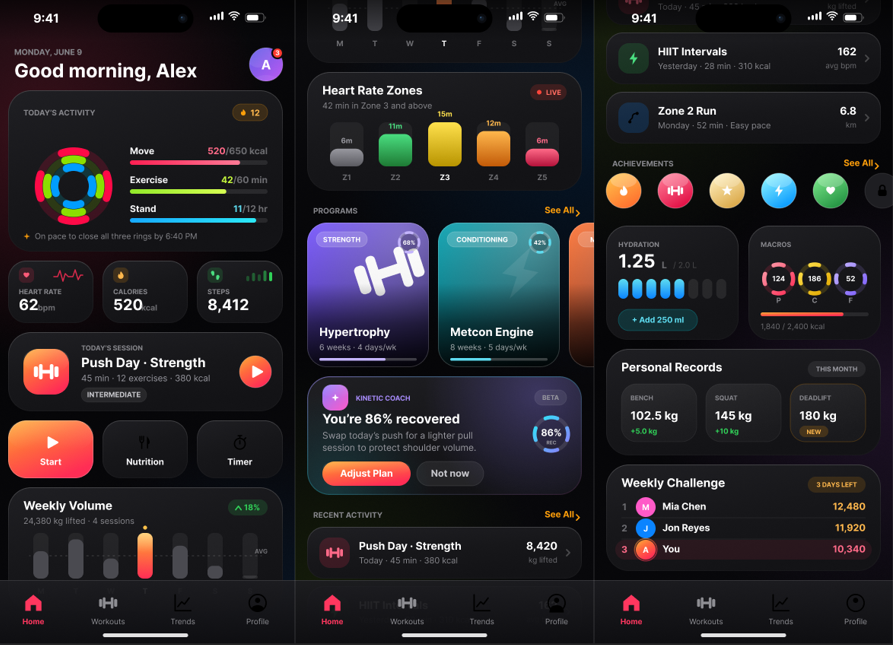
\includegraphics[width=5.5in]{screen.png}
    \caption{Alcedo Mobile Application Interface: Home Dashboard, Workout Execution, and Performance Analytics}
    \label{fig:app-screens}
\end{figure}

\subsection{System Architecture and Component Ecosystem}
The complete Alcedo platform is structured as a multi-tier client-server architecture consisting of a cross-platform mobile application, two specialized backend services, and a supplementary web portal:
\begin{enumerate}
    \item \textbf{Mobile Client Application (\textit{app/}):} Cross-platform frontend application developed using React Native 0.86, React 19, and Expo SDK 57 in TypeScript. It provides the primary user interface, local relational persistence via SQLite and Drizzle ORM, state management via Redux Toolkit, and secure token storage.
    \item \textbf{Modern Application Backend (\textit{backend-v2/}):} Modular RESTful server built on NestJS 11 and MongoDB 8 (Mongoose ODM). It handles user identity management, profile operations, workout synchronization contracts with idempotency keys, feature capability flags, and administrative site configurations.
    \item \textbf{Legacy Support Service (\textit{backend/}):} Pre-existing ASP.NET Core 10 backend supporting legacy SignalR real-time hubs and cryptographic messaging, maintained as an external dependency.
    \item \textbf{Web Portal (\textit{website/}):} Supplementary web interface built on Next.js 16 and Tailwind CSS for account management and administrative configurations.
\end{enumerate}

The high-level architectural relationship between the mobile client and supporting backend services is depicted in Figure~\ref{fig:sys-arch-flow}.

\begin{figure}[htbp]
    \centering
    \framebox[\textwidth]{
        \begin{minipage}{0.92\textwidth}
        \vspace{8pt}
        \centering
        \textbf{[Client Layer --- Mobile Device (iOS / Android)]}\\[3pt]
        \textit{Expo SDK 57 / React Native 0.86 (TypeScript 6.0)}\\
        \fbox{Expo Router Routes (24 Screens)} $\longrightarrow$ \fbox{Redux Toolkit (11 Slices)} $\longrightarrow$ \fbox{SQLite + Drizzle ORM (17 Tables)}\\
        \fbox{SecureStore (JWT Tokens)} $\longleftrightarrow$ \fbox{Authenticated Fetch Client (Single-Flight 401 Refresh)}\\[8pt]
        $\Big\Downarrow$ \textit{HTTPS / REST (Dual Base-URL Routing)} $\Big\Downarrow$\\[8pt]
        \begin{tabular}{c@{\hspace{0.4in}}c}
            \textbf{[Modern Backend Tier]} & \textbf{[Legacy Backend Tier]} \\
            \fbox{\parbox{2.3in}{\centering \textbf{backend-v2 (NestJS 11 + MongoDB)}\\
            User Management (\textit{/api/users/me})\\
            Workout Sync Contracts (\textit{/api/workouts})\\
            Feature Flags (\textit{/api/features})\\
            Admin Config (AES-256-GCM)}} &
            \fbox{\parbox{2.3in}{\centering \textbf{backend (.NET Core 10 + Postgres)}\\
            SignalR AI Chat Hubs\\
            Legacy Social Messaging\\
            Pre-existing Upstream Baseline}}
        \end{tabular}
        \vspace{8pt}
        \end{minipage}
    }
    \caption{Architectural Block Diagram and Data Flow of Project Alcedo}
    \label{fig:sys-arch-flow}
\end{figure}

\subsection{Technology Stack Summary}
The technological stack utilized across the design, implementation, and verification of Project Alcedo is detailed in Table~\ref{tab:tech-stack}.

\begin{table}[htbp]
    \centering
    \caption{Technology Stack of Project Alcedo}
    \label{tab:tech-stack}
    \begin{tabular}{|l|l|p{3.3in}|}
        \hline
        \textbf{Layer / Domain} & \textbf{Technology} & \textbf{Role and Architectural Function} \\
        \hline
        Mobile Framework & React Native 0.86 & Native cross-platform rendering engine \\
        Application Runtime & Expo SDK 57 & Unified build tooling, APIs, and Hermes engine \\
        Language & TypeScript 6.0 & Compile-time type safety across client and server \\
        Navigation Engine & Expo Router 57 & Declarative, file-based routing and deep-linking \\
        State Management & Redux Toolkit & Predictable single source of truth with middleware \\
        Local Embedded DB & SQLite & Embedded ACID-compliant client database engine \\
        Client-Side ORM & Drizzle ORM & Type-safe relational schema modeling and migrations \\
        Secure Storage & Expo SecureStore & Hardware-backed Keychain/KeyStore cryptographic vault \\
        Backend Framework & NestJS 11 & Modular, enterprise-grade TypeScript server \\
        Database Engine & MongoDB 8 & Scalable document-oriented NoSQL database \\
        Server-Side ODM & Mongoose 8 & Schema validation, indexing, and data models \\
        Testing Tooling & Vitest / Jest & Unit testing, component simulation, and API specs \\
        Static Code Analysis & Oxlint / ESLint & Code style enforcement, formatting, and linting \\
        \hline
    \end{tabular}
\end{table}

% ---------------------------------------------------------------------
\section{Tasks/Activities Performed}
This section provides an in-depth technical discussion of the software engineering activities executed during the internship, organized by architectural domain.

\subsection{Development Environment and Tooling Configuration}
The initial phase required configuring a standardized, reproducible mobile development environment. The client application configuration is defined in \textit{app/package.json} under the private package name \textit{alcedo-react}. 

Key development tooling configurations included:
\begin{itemize}
    \item \textbf{TypeScript Configuration:} Enforcing strict compiler checks via \textit{tsconfig.json} with \textit{strict: true}, \textit{strictNullChecks: true}, and \textit{noUncheckedIndexedAccess: true}. Path mapping aliases were established to decouple module resolution (e.g., \textit{@/*} mapping to \textit{src/*}).
    \item \textbf{Metro and Babel Bundler Setup:} Configured Metro bundler with SVG transformer plugins and path shims supporting styled-components on the Hermes JavaScript engine.
    \item \textbf{Static Analysis Tooling:} Integrated Oxlint and ESLint pipelines paired with Oxfmt formatters to enforce code hygiene and eliminate formatting variances across development commits.
\end{itemize}

\subsection{Reusable Interface Components and Design System}
To ensure interface consistency across 24 screens, a comprehensive foundation component library comprising 82 modular component files was constructed under \textit{app/src/components/presentation/foundation/}. 

The design system is anchored by the centralized design token specification in \textit{app/src/styles/theme.ts} (spanning 947 lines of code and 192 named typography definitions). The design tokens formalize:
\begin{itemize}
    \item \textbf{Color Palettes:} Semantic definitions for primary brand accents, container surfaces, borders, error states, and high-contrast text across Light, Dark, and true-black OLED display modes.
    \item \textbf{Typography Scale:} Responsive typographic hierarchies with explicit font sizes, line heights, and weights for display headers, section titles, card labels, and data tabular numbers.
    \item \textbf{Component Library:} Standardized atomic controls including \textit{AppButton} (primary, tonal, outlined, text variants), \textit{Card} containers, form input text fields with validation states, sheet selection dialogs, modal pickers, chip filters, and custom SVG bottom tab bar icons.
\end{itemize}

\subsection{Navigation and Screen Implementation}
Application navigation was implemented using Expo Router under \textit{app/src/app/}, organizing 49 individual route files into a cohesive hierarchy. The application root is wrapped by a root stack navigator in \textit{\_layout.tsx}, orchestrating top-level modal screens (such as exercise search, workout editor, and diff-save) over the core tab navigator.

The bottom tab navigator organizes five distinct operational tabs:
\begin{enumerate}
    \item \textbf{Workout Tab (\textit{(session)}):} Hub for initiating planned workout sessions, logging live active workouts, inspecting set history, and reviewing post-workout accomplishment summaries.
    \item \textbf{Feed Tab (\textit{feed}):} Displays social timeline posts, shared workout accomplishments, user profiles, and post details.
    \item \textbf{Stats Tab (\textit{stats}):} Analytical dashboards presenting longitudinal volume heatmaps, personal record progression, and exercise-specific strength curves.
    \item \textbf{History Tab (\textit{history}):} Interactive monthly training calendars, historical session review cards, and historical workout log editors.
    \item \textbf{Settings Tab (\textit{settings}):} Comprehensive configuration hub encompassing user profile management, display theme selectors, measurement unit toggles, local backup export/import tools, and backend connection diagnostic editors.
\end{enumerate}

A comprehensive inventory of the twenty-four primary tracked application screens is presented in Table~\ref{tab:screen-inventory}.

\begin{table}[htbp]
    \centering
    \caption{Primary Application Screen Inventory and Route Mapping}
    \label{tab:screen-inventory}
    \begin{tabular}{|c|l|l|p{2.6in}|}
        \hline
        \textbf{No.} & \textbf{Screen Identifier} & \textbf{Tab / Route Path} & \textbf{Functional Purpose} \\
        \hline
        1 & Home Dashboard & \textit{(session)/index} & Workout streaks, quick start, active plans \\
        2 & Active Workout & \textit{(session)/session/index} & Live set logging, rest timer, exercise swap \\
        3 & Post-Workout Summary & \textit{(session)/session/post} & Volume totals, PR badges, session notes \\
        4 & Workout Editor & \textit{workout-editor} & Blueprint builder, target reps/sets editor \\
        5 & Exercise Editor & \textit{exercise-editor} & Custom exercise name, muscle groups, equipment \\
        6 & Plan Diff-Save & \textit{diff-save} & Visual plan diffing and update reconciliation \\
        7 & Exercise Search & \textit{exercise-search} & Filtered catalog search by equipment and muscle \\
        8 & Exercise History & \textit{exercise-history} & Historical 1RM trends and set log history \\
        9 & Manage Exercises & \textit{settings/manage-exercises} & Custom exercise library administration \\
        10 & Feed Timeline & \textit{feed/index} & Community timeline and post feed \\
        11 & Feed Post Detail & \textit{feed/item/[id]} & Post inspection, reactions, and comments \\
        12 & Feed Share Composer & \textit{feed/share} & Share workout accomplishments to feed \\
        13 & Profile Editor & \textit{feed/profile-editor} & User display name, bio, and avatar settings \\
        14 & Shared Item Detail & \textit{feed/shared-item/[id]} & Deep-linked shared workout inspection \\
        15 & History Calendar & \textit{history/index} & Monthly workout calendar and week list \\
        16 & History Session Edit & \textit{history/edit} & Retroactive editing of completed workouts \\
        17 & Trends Dashboard & \textit{stats/index} & Volume heatmaps and weekly frequency graphs \\
        18 & Exercise Stats List & \textit{stats/exercise-list} & Per-exercise performance metric list \\
        19 & Expanded Stats & \textit{stats/expanded-weighted} & Detailed graphical progression curves \\
        20 & Settings Home & \textit{settings/index} & Primary user configuration hub \\
        21 & Preferences & \textit{settings/preferences} & Units (kg/lb), sound, and rest timer options \\
        22 & Notifications & \textit{settings/notifications} & Workout reminders and system alert toggles \\
        23 & Backup and Restore & \textit{settings/backup-and-restore} & Local JSON export/import and cloud sync \\
        24 & Backend Diagnostics & \textit{settings/backends/index} & Multi-server routing and capability probe \\
        \hline
    \end{tabular}
\end{table}

\subsection{State Management with Redux Toolkit}
Client-side operational state was architected using Redux Toolkit (RTK) across 11 domain slices located in \textit{app/src/store/slices/}. The store maintains independent state slices for:
\begin{itemize}
    \item \textit{Session Slice:} Active workout state, current exercise index, completed sets, active rest timer countdown, and session pause states.
    \item \textit{History Slice:} Cached completed workout summaries, calendar dates, and query filters.
    \item \textit{Exercises Slice:} Cached exercise definitions, user-created custom movements, and search indices.
    \item \textit{Preferences Slice:} User interface configurations, active color theme (dark/light/OLED), measurement units, and timer preferences.
    \item \textit{Backends Slice:} Registered server endpoints, active URL assignments, and probed feature availability flags.
    \item \textit{Auth Slice:} Active session state, authenticated user metadata, and token validity flags.
\end{itemize}

To coordinate complex asynchronous workflows without cluttering UI components, a custom listener middleware (\textit{addEffect}) was configured. The middleware intercepts specific action dispatches (e.g., completing a set or updating preferences) and triggers non-blocking secondary effects, including atomic SQLite persistence and cache invalidation.

\subsection{Local Data Storage, SQLite, and Drizzle ORM}
To deliver a true offline-first user experience, local persistence was implemented using an embedded SQLite database managed via Drizzle ORM under \textit{app/src/db/}. The database schema comprises 17 relational tables, organized with strict foreign key constraints and indexed queries.

The database tables encompass:
\begin{itemize}
    \item Core workout tables: \textit{sessions}, \textit{recorded\_exercises}, \textit{recorded\_sets}, \textit{cardio\_records}.
    \item Blueprint planning tables: \textit{program\_blueprints}, \textit{session\_blueprints}, \textit{exercise\_blueprints}, \textit{set\_blueprints}.
    \item Exercise definitions: \textit{exercise\_descriptors}, \textit{muscle\_groups}, \textit{equipment\_categories}.
    \item Synchronization and metadata: \textit{sync\_journal}, \textit{tombstones}, \textit{schema\_migrations}.
\end{itemize}

Schema evolution is governed by nine sequential SQL migrations. When the application initializes, a database bootstrapper verifies the active user-version pragma, executes pending migrations within a transactional block, and verifies schema integrity. For hardware-backed secret management, sensitive JWT tokens are stored outside SQLite using \textit{Expo SecureStore}, ensuring cryptographic isolation.

\subsection{Frontend--Backend Integration and Security Lifecycle}
Client--server communication was engineered to satisfy strict security and reliability standards. Network requests to the modern backend are mediated by a centralized client wrapper (\textit{authenticated-fetch.ts}). 

The integration architecture implements key security mechanisms:
\begin{itemize}
    \item \textbf{Stateless Token Injection:} Outgoing HTTP requests automatically inject the stored JWT access token into the standard \textit{Authorization: Bearer <token>} header.
    \item \textbf{Single-Flight 401 Refresh Interceptor:} When an access token expires, backend endpoints respond with HTTP 401 Unauthorized. The \textit{authenticated-fetch} wrapper intercepts this response, pauses concurrent outgoing network requests via an internal promise-based mutex, executes a single refresh request to \textit{/api/auth/refresh} using the securely stored refresh token, updates the token cache, and replays the queued requests. This pattern prevents duplicate, racing refresh requests when multiple UI queries fail concurrently.
    \item \textbf{Backend Capability Discovery:} The mobile client queries \textit{GET /api/features} through \textit{backend-probe.ts} to evaluate dynamic server capabilities (such as feed availability, backup support, and AI planning), gracefully adapting the client interface based on active server flags.
\end{itemize}

\subsection{User Management Module}
The User Management module in \textit{backend-v2/src/users/} provides profile management services for authenticated gym members. Developed with NestJS and MongoDB, the module implements:
\begin{itemize}
    \item Profile data retrieval via \textit{GET /api/users/me}, returning the member's profile attributes, account creation timestamp, and subscription entitlement status.
    \item Profile updates via \textit{PATCH /api/users/me}, allowing members to update display names, bio descriptions, and user preferences.
    \item Strict request validation enforced via class-validator DTOs (\textit{UpdateUserDto}), sanitizing inputs and rejecting malformed payloads before database execution.
\end{itemize}

\subsection{Workout Management and Synchronization Contracts}
The Workout Management service in \textit{backend-v2/src/workouts/} implements the server-side business logic for storing, validating, and synchronizing gym workout sessions.

Key technical components include:
\begin{itemize}
    \item \textbf{Workout CRUD Endpoints:} Endpoints for creating, fetching, modifying, and soft-deleting workout session documents.
    \item \textbf{Compare-and-Set Versioning:} Each workout document incorporates a monotonic version integer. Updates must present the matching expected version, preventing accidental overwrite of concurrent edits.
    \item \textbf{Soft Deletes and Tombstones:} Deleted sessions generate server-side tombstone records containing deletion timestamps, ensuring downstream synchronization cycles can reliably propagate deletions to client databases.
    \item \textbf{Batch Synchronization Contracts:} The backend exposes batch push and pull endpoints (\textit{/api/workouts/sync}) featuring idempotency key tracking. While the mobile client's production runtime currently executes local workout storage with client-side preparation, the backend sync contracts were validated and prepared for future enterprise multi-device replication.
\end{itemize}

\subsection{Feature Management and Runtime Configuration}
Feature Management is implemented through a two-tiered system operating across backend-v2 and the mobile client:
\begin{enumerate}
    \item \textbf{Public Feature Capability Flags:} The endpoint \textit{GET /api/features} distributes a public feature map reporting boolean availability flags (e.g., \textit{feed}, \textit{aiPlanner}, \textit{backup}, \textit{sharing}). The mobile app's \textit{backend-probe.ts} consumes this endpoint to adapt the UI dynamically.
    \item \textbf{Encrypted Site Configuration:} An administrative configuration service in \textit{backend-v2/src/site-config/} manages an allowlist of 16 system configuration keys. Sensitive secrets (such as external API keys) are encrypted at rest using AES-256-GCM authenticated encryption and masked during administrative read operations.
\end{enumerate}

\subsection{Testing, Quality Assurance, and Debugging}
Quality assurance was conducted systematically throughout development, combining automated unit tests, component simulations, static analysis, and emulator verification. The test suite distribution across system layers is summarized in Table~\ref{tab:test-distribution}.

\begin{table}[htbp]
    \centering
    \caption{Automated Quality Assurance and Test Suites by System Layer}
    \label{tab:test-distribution}
    \begin{tabular}{|l|l|c|p{2.8in}|}
        \hline
        \textbf{Layer} & \textbf{Framework} & \textbf{Suites / Specs} & \textbf{Verification Scope} \\
        \hline
        Mobile Client (\textit{app}) & Vitest & 140 Spec Files & Component simulations (51), Redux store (34), data models (25), services (19), utils (7), database (4) \\
        \hline
        Mobile Property Tests & Fast-Check & Embedded & Generative property tests for workout calculation and math \\
        \hline
        Mobile E2E Workflows & Maestro & 6 Flow Specs & Critical user journeys: onboard, log workout, view history \\
        \hline
        Backend Service & Jest & 19 Test Suites & 194 test blocks covering users, workouts, auth, and features \\
        \hline
        Static Type Checking & TypeScript & Whole Project & Strict mode compilation checking zero type errors \\
        \hline
        Code Linter / Formatter & Oxlint / ESLint & Whole Project & Code style, hook dependencies, and formatting checks \\
        \hline
    \end{tabular}
\end{table}

Quality gates were executed manually prior to commit integration, verifying typecheck cleanliness, lint passing, and test suite execution. Commit messages systematically recorded running test totals (progressing from 1,472 to over 2,140 passing tests) and documented verification boundaries.

\subsection{Version Control and Branch Management Workflow}
Software development followed disciplined Git version control workflows. Work was structured using feature branches, conventional commit semantics, and structured commit bodies detailing specific file modifications, executed test commands, and verification outputs. 

During major branch integrations, formal merge programmes were executed using documented merge ledgers (\textit{merge\_ledger.md}) and hazard registers. Pre-merge snapshots and safety tags were created to mitigate regression risks, ensuring clean branch consolidation across multi-thousand-line updates without architectural degradation.